\documentclass{beamer}

\usecolortheme[dark,accent=cyan]{solarized}

\beamertemplatenavigationsymbolsempty

\usepackage{graphicx}
\usepackage{hyperref}
\usepackage{colortbl, xcolor}
\usepackage{booktabs}
\usepackage{varwidth}

\usepackage{tikz}
\usetikzlibrary{calc}
\usepackage{minted}

\definecolor{DarkGray}{gray}{0.1}
\definecolor{DarkGray}{gray}{0.1}
\usemintedstyle{native}

\theoremstyle{definition}
\newtheorem{defn}{Definition}

\title{Accessing open research literature with Python}
\author{Nikoleta Glynatsi}
\date{2017-02}
\institute[]
{
\begin{center}
    
\includegraphics[width=.15\textwidth]{static/pycon-namibia.png}
\end{center}
}

\begin{document}

\frame{\titlepage}

\begin{frame}{About me}
    \begin{center}
    
\includegraphics[width=0.24\textwidth]{static/cardiff_uni_logo.jpg}\hspace{10pt}
    
\includegraphics[width=0.24\textwidth]{static/axelrod-logo.png}

    
\includegraphics[width=0.24\textwidth]{static/ssi-logo.png} \hspace{10pt}
    
\includegraphics[width=0.24\textwidth]{static/phoenix-logo.jpg}
    \end{center}
\end{frame}

\begin{frame}{}
    \begin{center}
       \begin{defn}A \textbf{literature review} is a search and evaluation of
       the available literature in your given subject or chosen topic area. \\
       -Royal Literary Fund
       \end{defn}
    \end{center}
\end{frame}

\begin{frame}
    \begin{center}
       \begin{defn}\textbf{Web Scraping} is a technique employed to extract large
            amounts of data from websites. - WebHarvy
       \end{defn}
    \end{center}
\end{frame}

\begin{frame}
    \begin{center}
    \begin{itemize}
        \item Literature Review;
        \item World Wide Web;
        \item Web Scraping;
    \end{itemize}
    \end{center}
\end{frame}

\begin{frame}{Arcas}
\begin{center}
    \small{https://github.com/Nikoleta-v3/Arcas}
\end{center}
\end{frame}

\begin{frame}[fragile]{Arcas}
    \begin{minted}
    [
    framesep=4mm,
    baselinestretch=1.2,
    bgcolor=DarkGray,
    fontsize=\footnotesize,
    ]
    {python}
 pip install arcas
    \end{minted}
    \hspace{10mm}
    \pause
    \begin{minted}
    [
    framesep=4mm,
    baselinestretch=1.2,
    bgcolor=DarkGray,
    fontsize=\footnotesize,
    ]
    {python}
 git clone git@github.com:Nikoleta-v3/Arcas.git
 python setup.py develop
    \end{minted}
\end{frame}

\begin{frame}[fragile]{Arcas}
    \begin{minted}
    [
    framesep=4mm,
    baselinestretch=1.2,
    bgcolor=DarkGray,
    fontsize=\footnotesize,
    ]
    {python}
 arcas_scrape -p arxiv -t "Prisoner's Dilemma" -y 2014 -r 1
    \end{minted}
    \hspace{10mm}
    \pause
    \begin{minted}
    [
    framesep=2mm,
    baselinestretch=1.2,
    bgcolor=DarkGray,
    fontsize=\footnotesize,
    ]
    {python}
 arcas_scrape -p ieee -t "Prisoner Dilemma" -a "Nowak" -y 2014
 ... -r 1 -s 2
    \end{minted}
    \hspace{10mm}
    \pause
    \begin{minted}
    [
    framesep=2mm,
    baselinestretch=1.2,
    bgcolor=DarkGray,
    fontsize=\footnotesize,
    ]
    {python}
 arcas_scrape -p ieee -b "game theory" -t "Prisoner Dilemma"
 ... -a "Nowak" -y 2014 -r 1 -s 2
    \end{minted}
\end{frame}

\begin{frame}[fragile]{Results}
    \begin{minted}
        [
        framesep=2mm,
        baselinestretch=1,
        bgcolor=DarkGray,
        fontsize=\footnotesize,
        ]
        {python}
{
"key":{"0":"Deng2014","1":"Deng2014","2":"Deng2014"},
"unique_key":{"0":"3369e749ce1c92062806e7fa3c41c90e",
              "1":"3369e749ce1c92062806e7fa3c41c90e",
              "2":"3369e749ce1c92062806e7fa3c41c90e"},
"title":{"0":"Generalized prisoner's dilemma",
         "1":"Generalized prisoner's dilemma",
         "2":"Generalized prisoner's dilemma"},
"author":{"0":"Xinyang Deng","1":"Qi Liu","2":"Yong Deng"},
"abstract":{"0":"  Prisoner's dilemma has been ...",
            "1":"  Prisoner's dilemma has been ...",
            "2":"  Prisoner's dilemma has been ..."},
"date":{"0":2014,"1":2014, "2":2014},
"journal":{"0":"arXiv","1":"arXiv","2":"arXiv"},
"provenance":{"0":"arXiv","1":"arXiv","2":"arXiv"}
}
     \end{minted}
\end{frame}


\begin{frame}
\begin{center}
\begin{figure}[H]
		\documentclass{standalone}

\usepackage{tikz}
\usepackage{standalone}
\usetikzlibrary{calc}
\usetikzlibrary{decorations.pathmorphing}
\usetikzlibrary{fit}                    % fitting shapes to coordinates
\usetikzlibrary{backgrounds}    % drawing the background after the foreground

\tikzstyle{background}=[orange, rectangle, draw, inner sep=0.2mm,
           rounded corners=1mm, ultra thick]

\begin{document}
\begin{tikzpicture}

\tikzstyle{state}=[minimum width=0.4cm, font=\boldmath];
    

    \node[ultra thick, draw=orange] (0) at (0, 0) [state] {tools.py};
    \node[ultra thick, draw=orange] (1) at (0, -2) [state] {doc/};

    \node[ultra thick, draw=orange] (2) at (0, -4) [state] {arcas.readthedocs.io/};

    \node[ultra thick] (3) at (4, 0) [state] {ieee};
    \node[ultra thick] (4) at (6, 0) [state] {nature};
    \node[ultra thick] (5) at (4, -1) [state] {arxiv};
    \node[ultra thick] (6) at (6, -1) [state] {$\dots$};  

    \node [background, inner sep=4mm, fit=(3) (4) (5) (6)] {};

    \node[ultra thick] (7) at (4, -3) [state] {test{\_}ieee};
    \node[ultra thick] (8) at (6, -3) [state] {test{\_}nature};
    \node[ultra thick] (9) at (4, -4) [state] {test{\_}arxiv};
    \node[ultra thick] (10) at (6, -4) [state] {$\dots$};  

    \node [background, fit=(7) (8) (9) (10)] {};

    \draw (1) edge[out=-90, in=90, -, thick, dotted] node [above] {} (2);

    \node [background, brown, inner sep=8mm, fit= (0) (1) (2) (3) (4) (5) (6) (7) (8) (9) (10)] {};

\end{tikzpicture}
\end{document}
\end{figure}
\end{center}
\end{frame}

\begin{frame}[fragile]
    \begin{minted}
        [
        framesep=2mm,
        baselinestretch=1,
        bgcolor=DarkGray,
        fontsize=\tiny,
        ]
        {python}
from arcas import *

def get_arguments(api, word, count):
    arguments = [{'-a': None, '-b': word, '-s': None,
                  '-r': count, '-y': None, '-t': None},
    return arguments

def main_program(arguments):
    parameters = pp.parameters_fix(arguments=arguments)
    url = pp.create_url_search(parameters=parameters)
    response = pp.make_request(url)
    root = pp.get_root(response)
    article = pp.parse(root)
    return article
    \end{minted}
    \pause
    \begin{minted}
        [
        framesep=2mm,
        baselinestretch=1,
        bgcolor=DarkGray,
        fontsize=\tiny,
        ]
        {python}
words = ["prisoner's dilemma", "prisoners evolution", "prisoner dilemma", ...]
apis = {"ieee": Ieee, "nature": Nature, "arxiv": Arxiv, "springer": Springer, "plos": Plos}
list_apis = ['plos', 'arxiv', 'ieee', 'nature', 'springer']
count = 10
\end{minted}
    \pause
    \begin{minted}
        [
        framesep=2mm,
        baselinestretch=1,
        bgcolor=DarkGray,
        fontsize=\tiny,
        ]
        {python}
for wr in words:
    for p in list_apis:
        pp = apis[p]()

        arguments = get_arguments(p, wr, count)
        raw_articles = main_program(arg)

        df = pp.to_dataframe(raw_article)
        pp.export(dfs, filename='articles/{}-{}.json'.format(p, wr))
\end{minted}
\end{frame}

\begin{frame}
\begin{center}
\begin{figure}[]
        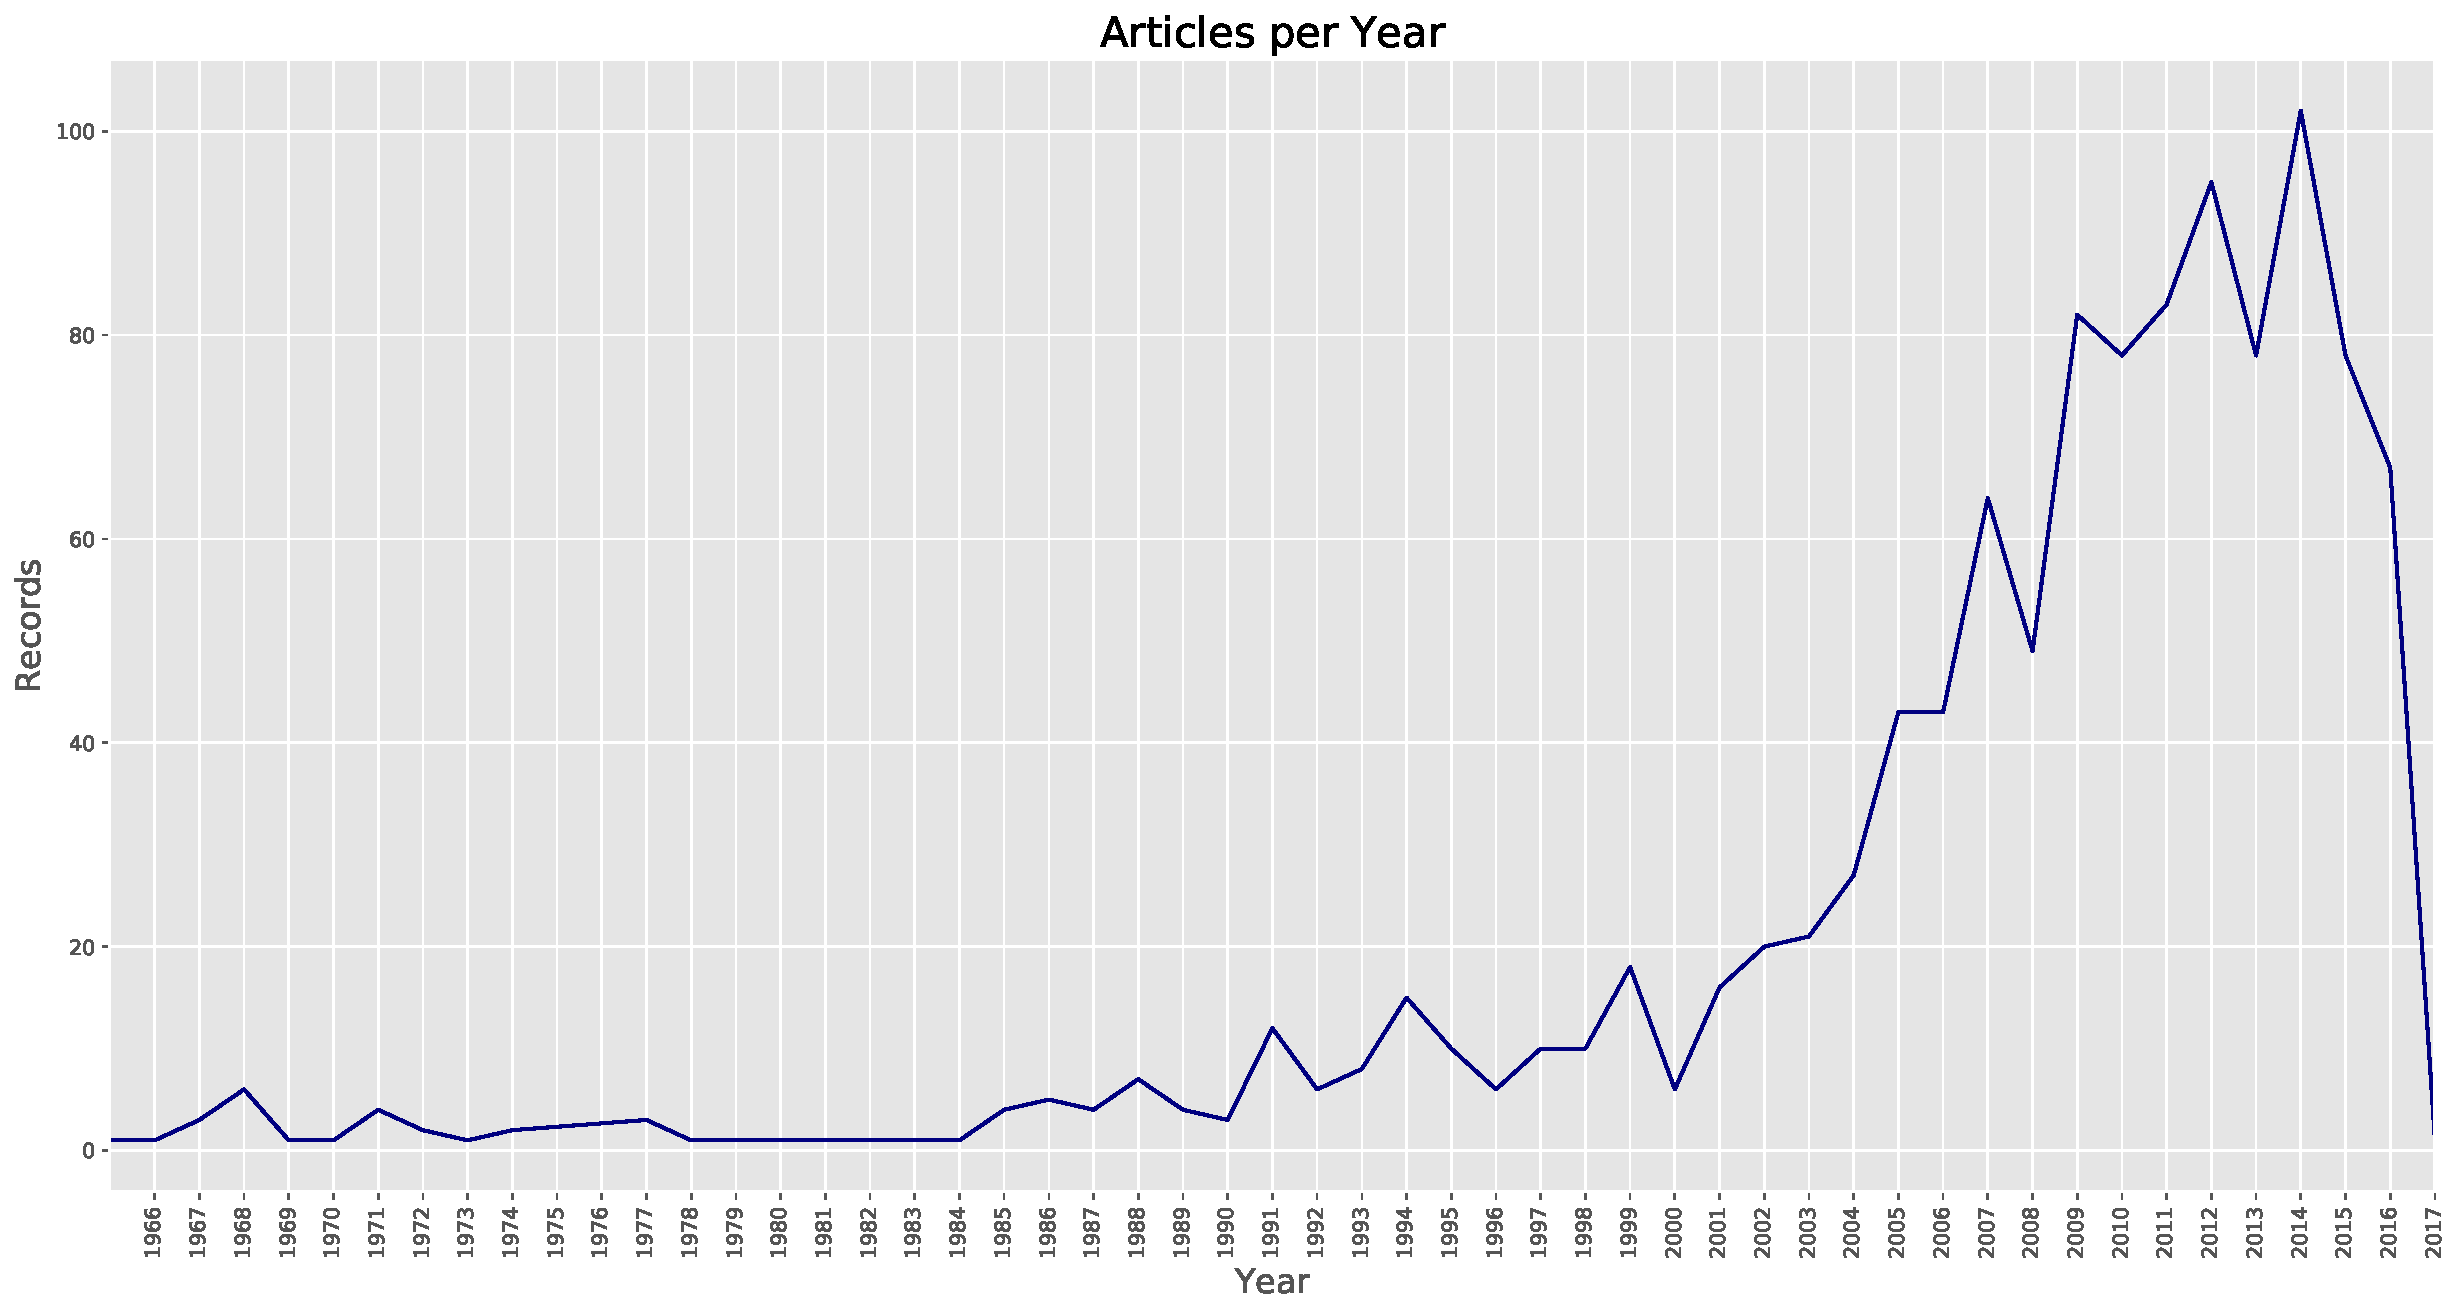
\includegraphics[width=\textwidth]{static/articles-year.pdf}
\end{figure}
\end{center}
\end{frame}

\begin{frame}
\begin{center}
\begin{figure}[]
        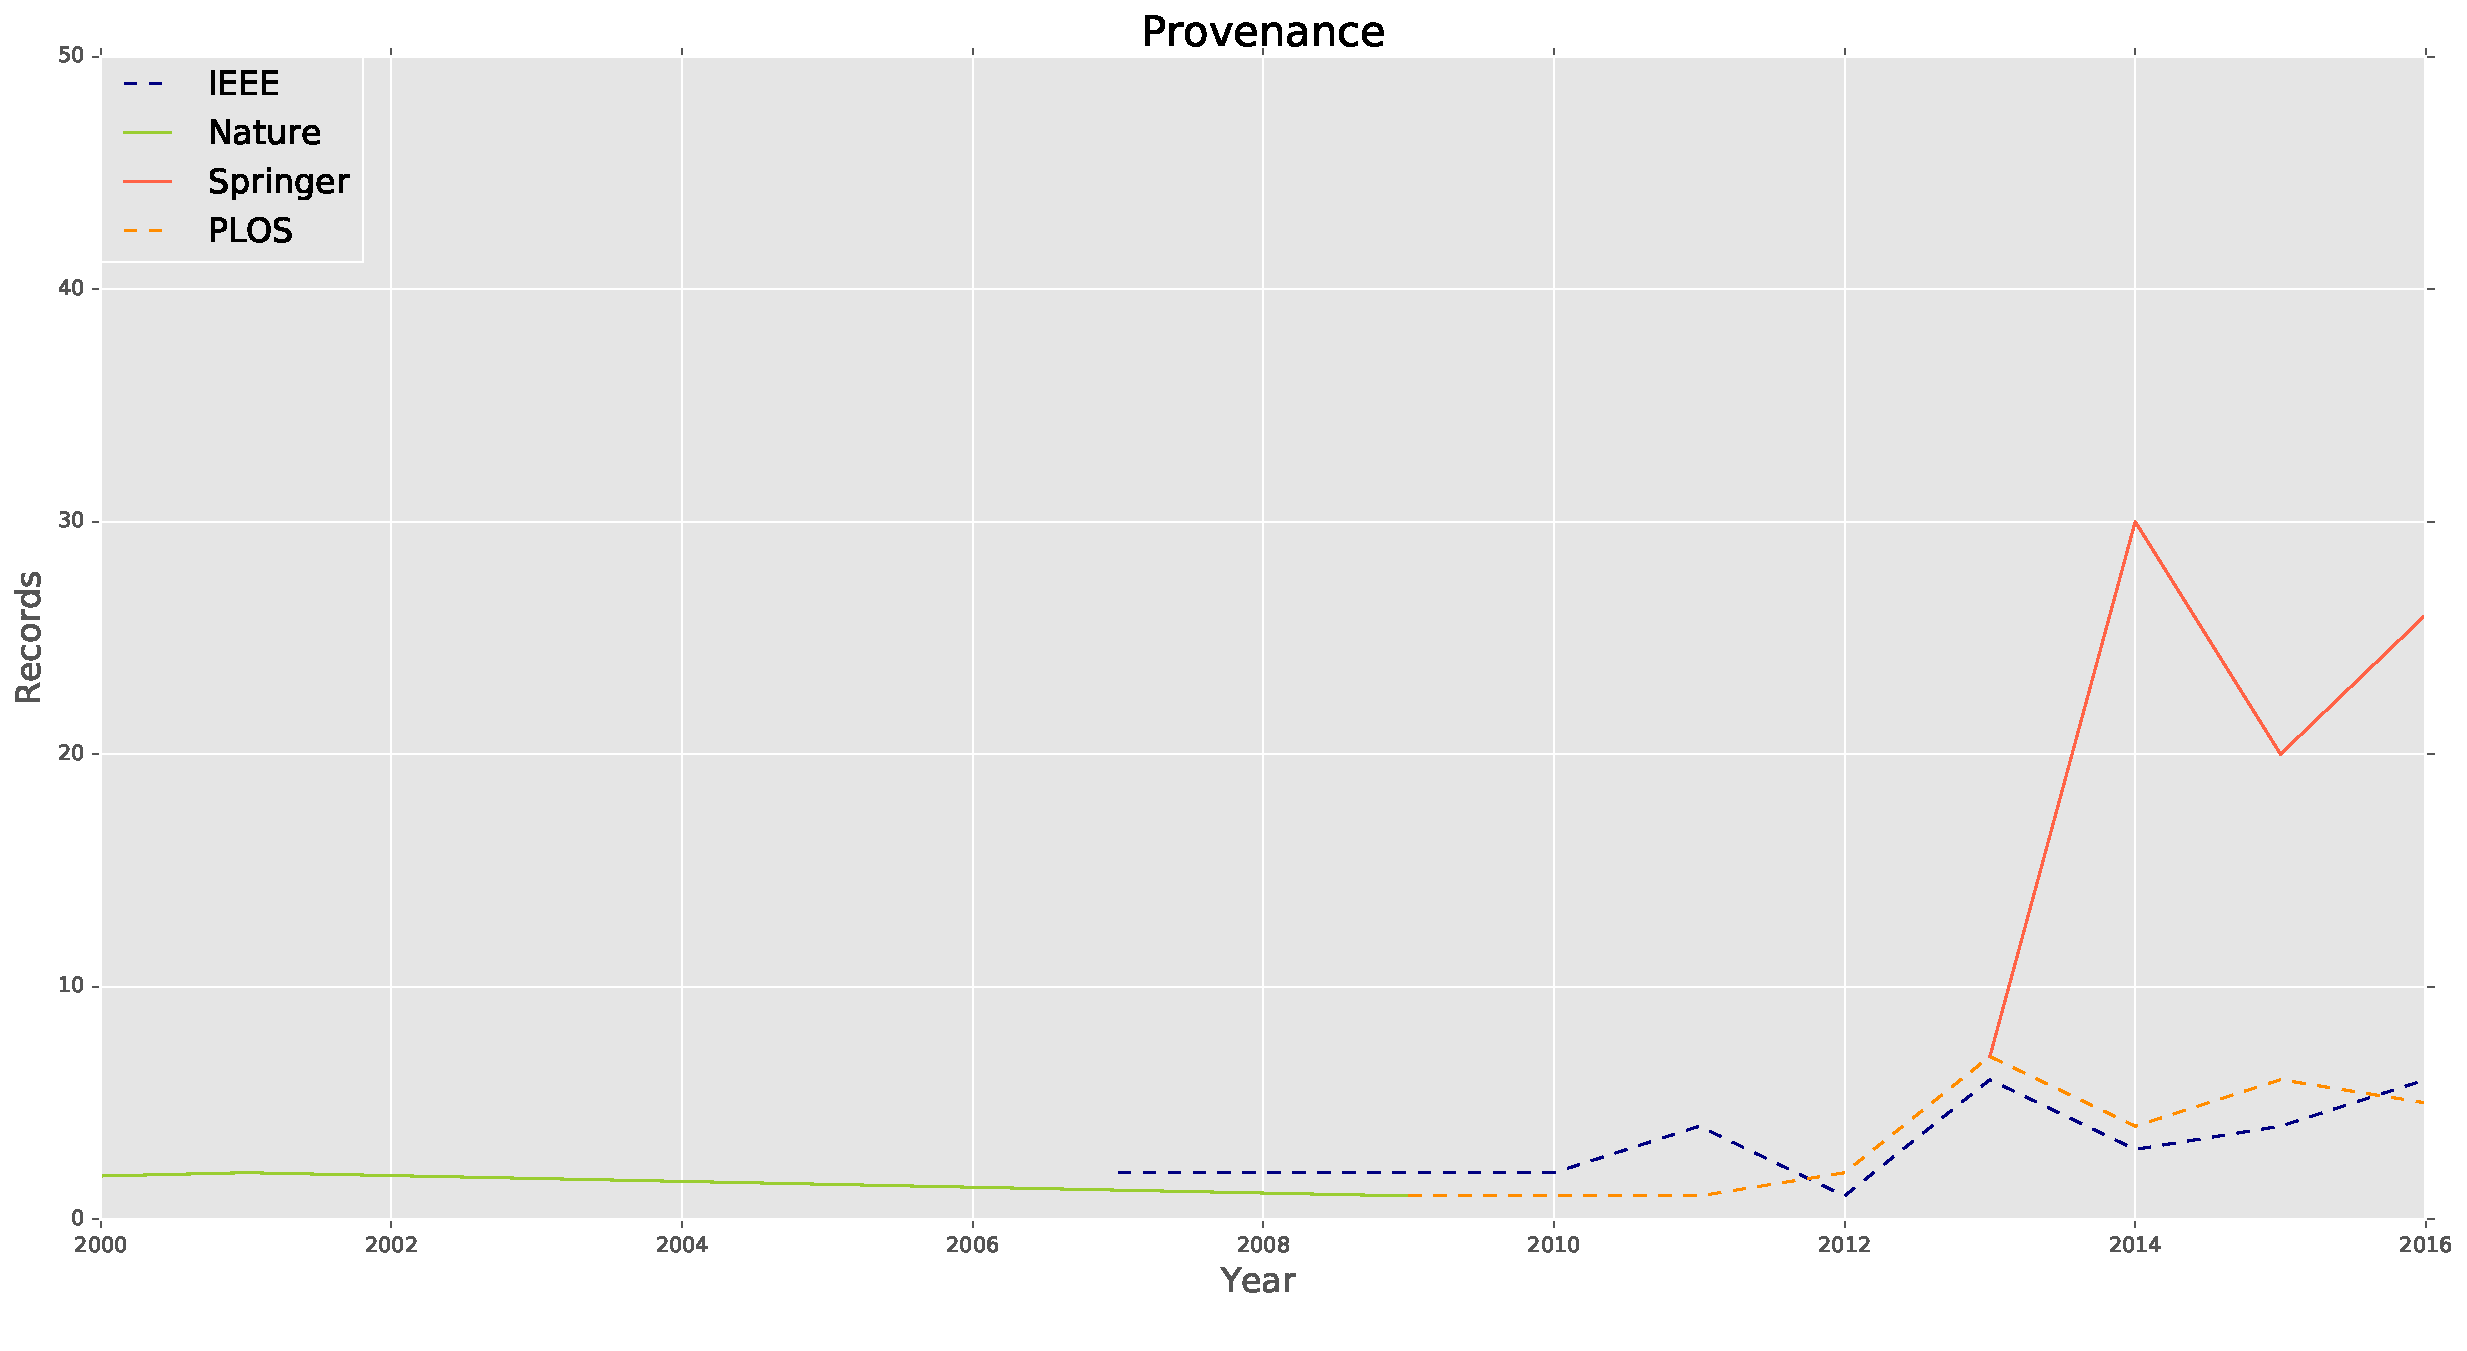
\includegraphics[width=\textwidth]{static/provenance.pdf}
\end{figure}
\end{center}
\end{frame}

\begin{frame}
	\begin{center}
		\huge{\textbf{}}\\~\\
		\small{@NikoletaGlyn}\\
		\small{https://github.com/Nikoleta-v3}\\
		\small{ttps://github.com/Nikoleta-v3/Arcas}
	\end{center}
\end{frame}

\end{document}




